\documentclass[aspectratio=169]{beamer}
\usetheme[minimal,]{tugraz2018}
%% Choose main theme variant:
% [standard]        % standard (default)
% [institute]       % with institute's graphical acronym on the left
% [minimal]         % with reduced visuals

%% Choose your font style:
%                   % Helvetica (default for Corporate Design)
% [webfont]         % Source Sans Pro (as used on tugraz.at)
% [nofont]          % no font loaded - Computer Modern Sans

%% Choose your department's color instead of TU Graz red (optional):
% [arch]            %
% [bau]             %
% [etit]            %
% [mbww]            %
% [tcvp]            %
% [mpug]            %
% [infbio]          %

\usepackage[utf8]{inputenc}
\usepackage[english]{babel}

%% Enter presentation metadata
\title[Short Title]{Secure Classification as a Service}
\author{Peter Waldert}
\date{Presentation Event/Date}
\institute{IAIK}
\instituteurl{iaik.tugraz.at}

%% Logos
\institutelogo{beamerthemetugraz/institute/iaik}  % graphical acronym for [institute] theme (left margin)
% \additionallogo{figures/logo}  % additional institute/department logo (footline; optional)
% \logobar{Supported by: ...}  % sponsors (titlepage; optional)

\begin{document}
  \begin{frame}[plain]
    \maketitle
  \end{frame}

  \begin{frame}{Outline}
    \tableofcontents
  \end{frame}

  \section{Introduction}
  \begin{frame}{The frame title}
    A text frame
  \end{frame}

  \section{Content}
  \begin{frame}{Lists}
    \begin{itemize}
      \item First item
      \item Second item
      \item Third item
    \end{itemize}
  \end{frame}

  \begin{frame}{Numbered Lists and Pauses}
    \begin{enumerate}
      \item First item
            \begin{enumerate}
              \item First subitem
                    \begin{enumerate}
                      \item First
                      \item Second
                    \end{enumerate}
            \end{enumerate}
            \pause
      \item Second item
            \pause
      \item Third item
    \end{enumerate}
  \end{frame}

  \begin{frame}{An Image}
    \centering
    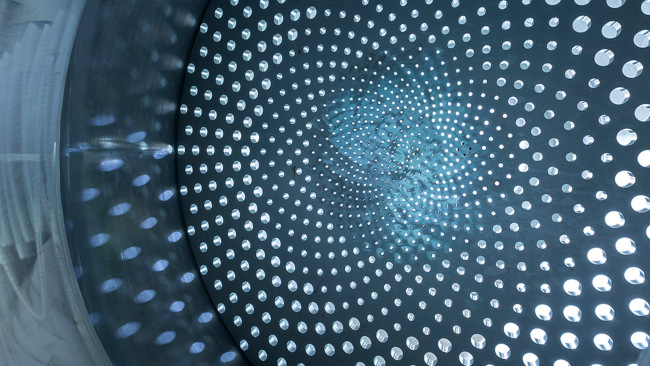
\includegraphics[height=0.6\textheight]{figures/photoexample-169}
  \end{frame}

  \section*{}
  \begin{frame}{Conclusion}
    ...
  \end{frame}

  %\begin{frame}[c,plain]
  \begin{frame}[c]
    \centering
    \Large Questions?
  \end{frame}
\end{document}
